\begin{figure*}[!t]
\centering
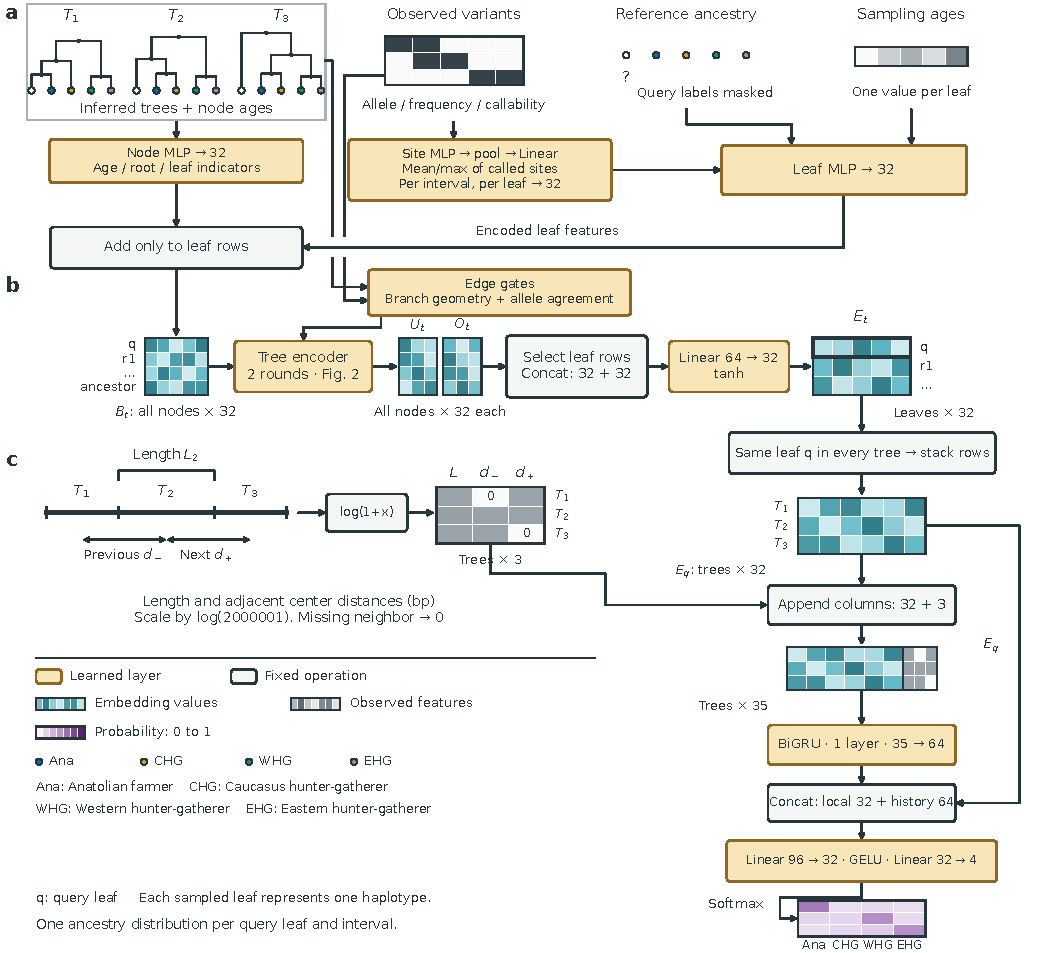
\includegraphics[width=\textwidth]{figures/TreeLoom_architecture.pdf}
\caption{TreeLoom predicts local ancestry for each query leaf and interval. Each sampled leaf represents one haplotype.
\textbf{a,} Node features initialize all nodes, including ancestors. Observed site features are encoded and pooled over called sites within each interval separately for each leaf. Reference labels and sampling ages join this pooled evidence, and the resulting features are added only to leaf rows. Query ancestry labels are masked. Branch geometry and observed allele--branch agreement supply learned message gates.
\textbf{b,} The two rounds of the tree encoder are expanded in Figure~\ref{fig:encoder}. Its output has upward and outside embeddings for every node. Selecting leaf rows, concatenating the two states and projecting gives a local leaf embedding of width 32.
\textbf{c,} Rows for the same query leaf are stacked in tree order. Interval length and distances to adjacent interval centers add three columns before the BiGRU. Its output joins the original local embedding for classification. Four ancestry classes illustrate the European condition. All matrix values and probabilities are schematic, not fitted results.}
\label{fig:architecture}
\end{figure*}
